\documentclass[11pt,a4paper]{article}

\usepackage[utf8]{inputenc}
\usepackage[T1]{fontenc}
\usepackage{lmodern}
\usepackage[spanish,es-tabla]{babel}
\spanishdecimal{.}  % decimal point everywhere, also in math (consistent with the tables)
\usepackage[a4paper,margin=2.2cm]{geometry}
\usepackage{microtype}
\usepackage{amsmath,amssymb}
\usepackage{booktabs}
\usepackage{graphicx}
\usepackage{xspace}
\usepackage{caption}
\usepackage{listings}
\usepackage{enumitem}
\usepackage[hidelinks]{hyperref}

\captionsetup{font=small,labelfont=bf}
\setlist{nosep,leftmargin=*}
\setlength{\parskip}{3pt}
\lstset{basicstyle=\ttfamily\scriptsize,frame=single,breaklines=true,columns=fullflexible,
        keepspaces=true,showstringspaces=false,aboveskip=4pt,belowskip=2pt}

% Every figure quoted in the text is a macro generated by python/report_data.py
% from benchmark.json and the result files; nothing is typed by hand in this file.
% Generated by python/report_data.py -- do not edit by hand.
\newcommand{\nTotal}{150\xspace}
\newcommand{\nTrain}{120\xspace}
\newcommand{\nTest}{30\xspace}
\newcommand{\nFeatures}{4\xspace}
\newcommand{\nClasses}{3\xspace}
\newcommand{\nHidden}{8\xspace}
\newcommand{\learningRate}{0.1\xspace}
\newcommand{\nEpochs}{1000\xspace}
\newcommand{\checkEpochs}{20\xspace}
\newcommand{\seedValue}{42\xspace}
\newcommand{\testFraction}{20\%\xspace}
\newcommand{\testSamplePct}{3.3\%\xspace}
\newcommand{\csvDigits}{17\xspace}
\newcommand{\lossTol}{\ensuremath{10^{-9}}\xspace}
\newcommand{\pageKB}{16\xspace}
\newcommand{\cppStd}{17\xspace}
\newcommand{\gradEps}{\ensuremath{10^{-6}}\xspace}
\newcommand{\gradTol}{\ensuremath{10^{-6}}\xspace}
\newcommand{\fwdTol}{\ensuremath{10^{-12}}\xspace}
\newcommand{\nParams}{67\xspace}
\newcommand{\cppTrainAcc}{97.50\%\xspace}
\newcommand{\cppTestAcc}{96.67\%\xspace}
\newcommand{\skTrainAcc}{97.50\%\xspace}
\newcommand{\skTestAcc}{96.67\%\xspace}
\newcommand{\cppTrainLoss}{0.0495\xspace}
\newcommand{\skTrainLoss}{0.0495\xspace}
\newcommand{\cppTestLoss}{0.0789\xspace}
\newcommand{\skTestLoss}{0.0789\xspace}
\newcommand{\initTrainLoss}{1.3618\xspace}
\newcommand{\testErrors}{1\xspace}
\newcommand{\testCorrect}{29\xspace}
\newcommand{\maxLossDiff}{\ensuremath{6.7\times10^{-16}}\xspace}
\newcommand{\zeroDiffEpochs}{153\xspace}
\newcommand{\initLossDiff}{\ensuremath{6.7\times10^{-16}}\xspace}
\newcommand{\probaDiff}{\ensuremath{2.2\times10^{-16}}\xspace}
\newcommand{\weightsDiff}{\ensuremath{1.1\times10^{-16}}\xspace}
\newcommand{\curveTwentyDiff}{\ensuremath{6.7\times10^{-16}}\xspace}
\newcommand{\gradcheckMaxRel}{\ensuremath{2.9\times10^{-9}}\xspace}
\newcommand{\gradcheckPoints}{2\xspace}
\newcommand{\nReps}{20\xspace}
\newcommand{\nWarmup}{2\xspace}
\newcommand{\nBlocks}{8\xspace}
\newcommand{\repsPerBlock}{5\xspace}
\newcommand{\blockOrder}{\texttt{C S S C C S S C}\xspace}
\newcommand{\cppMedianMs}{4.35\xspace}
\newcommand{\skMedianMs}{50.75\xspace}
\newcommand{\cppMeanMs}{4.35\xspace}
\newcommand{\skMeanMs}{50.72\xspace}
\newcommand{\cppStdMs}{0.09\xspace}
\newcommand{\skStdMs}{1.11\xspace}
\newcommand{\cppMinMs}{4.16\xspace}
\newcommand{\skMinMs}{48.79\xspace}
\newcommand{\cppMaxMs}{4.49\xspace}
\newcommand{\skMaxMs}{52.39\xspace}
\newcommand{\speedupMedian}{11.7\xspace}
\newcommand{\speedupBlockMin}{11.4\xspace}
\newcommand{\speedupBlockMax}{11.9\xspace}
\newcommand{\speedupHistMin}{10.4\xspace}
\newcommand{\speedupHistMax}{11.8\xspace}
\newcommand{\nHistoryRuns}{6\xspace}
\newcommand{\partialMedianMs}{423.7\xspace}
\newcommand{\partialOverFit}{8.3\xspace}
\newcommand{\cppPerEpochUs}{4.4\xspace}
\newcommand{\skPerEpochUs}{50.7\xspace}
\newcommand{\nMemRuns}{5\xspace}
\newcommand{\cppPeakMB}{2.03\xspace}
\newcommand{\skPeakMB}{160\xspace}
\newcommand{\memRatio}{79\xspace}
\newcommand{\cppGrowthKB}{49.2\xspace}
\newcommand{\skGrowthKB}{0\xspace}
\newcommand{\workspaceKB}{45\xspace}
\newcommand{\envCpu}{Apple M4\xspace}
\newcommand{\envCpus}{10\xspace}
\newcommand{\envRamGiB}{24\xspace}
\newcommand{\envOs}{macOS-27.0.1-arm64-arm-64bit-Mach-O\xspace}
\newcommand{\envCompiler}{Apple clang version 21.0.0 (clang-2100.3.34.2)\xspace}
\newcommand{\envFlags}{\texttt{-O3 -DNDEBUG -std=c++17 -arch arm64}\xspace}
\newcommand{\envEigen}{3.4.0\xspace}
\newcommand{\envPython}{3.14.8\xspace}
\newcommand{\envNumpy}{2.5.4\xspace}
\newcommand{\envSklearn}{1.9.1\xspace}
\newcommand{\envPower}{Now drawing from 'AC Power'\xspace}

\newcommand{\locCpp}{172\xspace}
\newcommand{\locPython}{40\xspace}
\newcommand{\locRatio}{4.3\xspace}
\newcommand{\locCppCore}{80\xspace}
\newcommand{\locPythonCore}{18\xspace}


\newcommand{\cpp}{C\texttt{++}\xspace}
\newcommand{\sk}{\textit{scikit-learn}\xspace}

\title{Red neuronal para Iris: implementaci\'on desde cero en \cpp (Eigen)\\frente a \sk}
\author{Juan Jos\'e M\'arquez\\Universidad Sergio Arboleda --- Redes Neuronales}
\date{Proyecto final}

\begin{document}
\maketitle

\begin{abstract}
Se implementa la misma red neuronal de una capa oculta en dos versiones, una escrita desde cero en \cpp con Eigen (propagaci\'on hacia adelante y hacia atr\'as) y otra con el \texttt{MLPClassifier} de \sk, y se comparan en el conjunto Iris. Ambas parten de los mismos datos, los mismos pesos iniciales y los mismos hiperpar\'ametros, de modo que siguen la misma trayectoria de entrenamiento: las curvas de p\'erdida difieren como m\'aximo en \maxLossDiff{} y las predicciones de prueba son id\'enticas. En esa igualdad de condiciones, la versi\'on en \cpp entrena \speedupMedian{}$\times$ m\'as r\'apido (mediana) y usa \memRatio{} veces menos memoria pico, pero necesita \locRatio{} veces m\'as l\'ineas de c\'odigo. El documento detalla la metodolog\'ia y sus limitaciones: el problema es diminuto y la aceleraci\'on est\'a dominada por el costo fijo de \textit{Python}.
\end{abstract}

\section{Introducci\'on}
El objetivo es comparar dos formas de obtener la misma red neuronal: programar la propagaci\'on hacia adelante y hacia atr\'as de forma expl\'icita (\cpp con Eigen~\cite{eigen}) o usar una biblioteca de alto nivel (\sk~\cite{pedregosa2011}). Los criterios son precisi\'on, p\'erdida, tiempo de ejecuci\'on, memoria, facilidad de implementaci\'on y ventajas y desventajas de cada enfoque.

Una comparaci\'on de tiempos solo tiene sentido si ambos programas hacen \emph{exactamente} el mismo c\'alculo. Por eso gran parte del trabajo consiste en garantizar y verificar la equivalencia (secci\'on~\ref{sec:equiv}) antes de medir. Todo el flujo se ejecuta con un solo comando (\texttt{uv run run\_all.py}), y las cifras, tablas y figuras de este documento se generan autom\'aticamente a partir de los resultados de esa ejecuci\'on.

\section{Datos y arquitectura}
Se usa el conjunto Iris~\cite{fisher1936}: \nTotal{} muestras, \nFeatures{} caracter\'isticas num\'ericas y \nClasses{} clases balanceadas. La divisi\'on es estratificada, con \testFraction{} para prueba (\nTrain{} muestras de entrenamiento y \nTest{} de prueba) y semilla \seedValue{}. Las caracter\'isticas se estandarizan con la media y la desviaci\'on est\'andar del conjunto de entrenamiento \'unicamente. Python exporta ambas particiones a CSV con \csvDigits{} cifras significativas, que reproducen exactamente cada \texttt{float64}, y el programa en \cpp lee esos mismos archivos.

La red tiene \nFeatures{} entradas, \nHidden{} neuronas ocultas con activaci\'on ReLU y \nClasses{} salidas con \textit{softmax}, es decir, \nParams{} par\'ametros. Los pesos iniciales se generan una sola vez (normal de He~\cite{he2015} para la capa oculta, normal de Glorot~\cite{glorot2010} para la de salida, sesgos nulos) y se exportan a CSV para que ambas versiones partan del mismo punto. La p\'erdida es la entrop\'ia cruzada media y el optimizador es descenso de gradiente de lote completo con tasa $\eta=\learningRate$ durante \nEpochs{} \'epocas.

\section{Implementaci\'on en \cpp}
\subsection{Ecuaciones}
Con $X\in\mathbb{R}^{N\times \nFeatures}$ ($N=\nTrain$), etiquetas $y_i$ y $Y$ su codificaci\'on \textit{one-hot}, la propagaci\'on hacia adelante es
\begin{align}
Z_1 &= XW_1+\mathbf{1}b_1^\top, & H &= \max(Z_1,0), \nonumber\\
Z_2 &= HW_2+\mathbf{1}b_2^\top, & P &= \operatorname{softmax}(Z_2)\ \text{(por filas)},\label{eq:fwd}\\
\mathcal{L} &= -\frac1N\sum_{i=1}^{N}\log P_{i,y_i}. \nonumber
\end{align}
La retropropagaci\'on~\cite{rumelhart1986,goodfellow2016} se reduce a
\begin{align}
dZ_2 &= \frac{P-Y}{N}, & dW_2 &= H^\top dZ_2, & db_2 &= \mathbf{1}^\top dZ_2,\nonumber\\
dH &= dZ_2W_2^\top, & dZ_1 &= dH\odot\mathbb{1}[Z_1>0], & dW_1 &= X^\top dZ_1,\quad db_1=\mathbf{1}^\top dZ_1,\label{eq:bwd}
\end{align}
y cada par\'ametro se actualiza con $\theta\leftarrow\theta-\eta\,d\theta$. La combinaci\'on \textit{softmax} y entrop\'ia cruzada colapsa en $dZ_2=(P-Y)/N$, y la derivada de ReLU vale $1$ donde $z>0$ y $0$ en el resto. El listado~\ref{lst:bwd} muestra la funci\'on real, extra\'ida del c\'odigo fuente.

\lstinputlisting[language=C++,caption={Retropropagaci\'on en \cpp (extracto de \texttt{network.hpp}).},label={lst:bwd}]{generated/listing_backward.cpp}

\subsection{Decisiones de dise\~no}
\begin{itemize}
\item \textbf{Referencias constantes.} \texttt{forward} y \texttt{backward} reciben los datos y los par\'ametros por \texttt{const\&} y solo escriben en el espacio de trabajo y en los gradientes; \'unicamente el paso de actualizaci\'on modifica los par\'ametros. As\'i se evitan copias de las matrices y el compilador garantiza que los datos de entrada no se alteran.
\item \textbf{Buffers preasignados.} Una estructura \texttt{Workspace} crea una sola vez todos los intermedios (\(Z_1,H,\) logits, probabilidades, \(dZ_2,dH,dZ_1\)), unos \workspaceKB{} KB, y \texttt{Grads} los gradientes. Cada \'epoca reutiliza esos buffers: las asignaciones a matrices del mismo tama\~no no reservan memoria, y \texttt{.noalias()} evita el temporal que Eigen crea por defecto en los productos. Un programa de verificaci\'on (\texttt{noalloc\_check}) corre las \nEpochs{} \'epocas con \texttt{EIGEN\_RUNTIME\_NO\_MALLOC} y falla ante cualquier reserva; forma parte de las pruebas.
\item \textbf{Estabilidad num\'erica.} El \textit{softmax} resta el m\'aximo de cada fila y la p\'erdida se calcula con \textit{log-sum-exp}, evitando desbordes de \texttt{exp}.
\item \textbf{Punto de registro de la p\'erdida.} La p\'erdida de cada \'epoca se toma en la propagaci\'on hacia adelante, antes de actualizar, que es donde \sk registra \texttt{loss\_curve\_}; las dos curvas son directamente comparables.
\item \textbf{Compilaci\'on.} CMake, \cpp\cppStd, \textit{Release} por defecto con los flags \envFlags; Eigen~\envEigen{} se busca en el sistema y, si no est\'a, se descarga con \texttt{FetchContent}. El proyecto abre directamente en Qt Creator.
\end{itemize}

\subsection{Verificaci\'on del gradiente}
El modo \texttt{--gradcheck} compara el gradiente anal\'itico con diferencias centrales, $\partial\mathcal{L}/\partial\theta_k\approx[\mathcal{L}(\theta_k+\varepsilon)-\mathcal{L}(\theta_k-\varepsilon)]/2\varepsilon$ con $\varepsilon=\gradEps$. El error relativo se mide por tensor, $\lVert a-n\rVert/(\lVert a\rVert+\lVert n\rVert)$; la versi\'on elemento a elemento es inestable donde el gradiente es casi nulo. Se prob\'o en \gradcheckPoints{} puntos (pesos iniciales y tras \checkEpochs{} \'epocas, con sesgos ya distintos de cero) y el peor error relativo fue \gradcheckMaxRel{}, muy por debajo del umbral de $\gradTol$.

\section{Implementaci\'on en Python}
La versi\'on de \sk usa \texttt{MLPClassifier} configurado para ser equivalente a la de \cpp (tabla~\ref{tab:config}); el listado~\ref{lst:model} es la funci\'on que lo construye.

\begin{table}[tbp]\centering\small
\caption{Configuraci\'on de equivalencia. La columna de \sk se lee del objeto real.}\label{tab:config}
\begin{tabular}{lp{4.1cm}p{5.6cm}}
\toprule
Aspecto & C++ (Eigen) & scikit-learn \\
\midrule
Arquitectura & 4--8--3 & \texttt{hidden\_layer\_sizes=(8,)} \\
Activación oculta & ReLU & \texttt{activation='relu'} \\
Salida y pérdida & softmax + entropía cruzada media & softmax + log-loss (implícitos) \\
Optimizador & descenso de gradiente por lote completo & \texttt{solver='sgd'} \\
Tamaño de lote & 120 & \texttt{batch\_size=120} \\
Tasa de aprendizaje & 0.1 & \texttt{learning\_rate\_init=0.1}, \texttt{learning\_rate='constant'} \\
Momentum & no & \texttt{momentum=0.0}, \texttt{nesterovs\_momentum=False} \\
Regularización $L_2$ & no & \texttt{alpha=0.0} \\
Orden de las muestras & fijo & \texttt{shuffle=False} \\
Criterios de parada & ninguno & \texttt{tol=0.0}, \texttt{early\_stopping=False}, \texttt{n\_iter\_no\_change=1001} \\
Pesos iniciales & CSV compartido & CSV compartido, copiados in situ a coefs\_ \\
Épocas & 1000 & \texttt{max\_iter} / llamadas a \texttt{partial\_fit} \\
Precisión numérica & \texttt{double} & \texttt{float64} \\
\bottomrule
\end{tabular}

\end{table}

\lstinputlisting[language=Python,caption={Construcci\'on del modelo de \sk.},label={lst:model}]{generated/listing_build_model.py}

\paragraph{\texttt{partial\_fit} frente a \texttt{warm\_start}.} \sk no permite inyectar los pesos iniciales al constructor. Se llama una vez a \texttt{partial\_fit}, que inicializa la red, y se sobrescriben \texttt{coefs\_} e \texttt{intercepts\_} \emph{in situ} con los pesos del CSV; reasignar las listas ser\'ia un error silencioso, porque el optimizador conserva referencias a los arreglos originales y entrenar\'ia esos. Desde ah\'i hay dos formas de entrenar:
\begin{itemize}
\item \texttt{partial\_fit} \emph{una vez por \'epoca}: da la trayectoria exacta, pero cada llamada revalida la entrada, as\'i que su tiempo mide sobre todo el costo de llamar a Python y se informa aparte, como sobrecarga.
\item \texttt{fit()} \emph{en una sola llamada} con \texttt{warm\_start=True}, que contin\'ua desde los pesos ya cargados sin reinicializarlos. Con \texttt{tol=0} y un \texttt{n\_iter\_no\_change} mayor que el n\'umero de \'epocas no hay parada anticipada. Este es el tiempo comparable con \cpp. Una prueba automatizada confirma que ambas rutas producen la misma curva de p\'erdida.
\end{itemize}

\section{Metodolog\'ia}
\subsection{Equivalencia}\label{sec:equiv}
Python exporta valores de referencia calculados con \sk y numpy, y el binario de \cpp los comprueba por s\'i mismo con tolerancia $\fwdTol$: la p\'erdida inicial coincide dentro de \initLossDiff{}, las probabilidades de salida dentro de \probaDiff{}, y tras \checkEpochs{} \'epocas de entrenamiento los pesos coinciden dentro de \weightsDiff{} y la curva de p\'erdida dentro de \curveTwentyDiff{}. Al final de cada ejecuci\'on completa, \texttt{run\_all.py} falla si la p\'erdida difiere en m\'as de $\lossTol$, si las curvas difieren en m\'as de esa cota o si cualquier exactitud o predicci\'on de prueba no es id\'entica.

\subsection{Benchmark}
\textbf{Tiempo.} Solo se cron\'ometra el entrenamiento. En \cpp, el binario repite el entrenamiento dentro del mismo proceso, recarga los pesos iniciales desde memoria en cada repetici\'on (fuera del cron\'ometro) y mide solo el bucle de \'epocas con \texttt{steady\_clock}. En \sk, cada repetici\'on crea un \texttt{MLPClassifier} nuevo y mide solo la llamada a \texttt{fit()}. Cada bloque descarta \nWarmup{} repeticiones de calentamiento y mide \repsPerBlock{}; se alternan \nBlocks{} bloques en orden \blockOrder{} (\texttt{C}=\cpp, \texttt{S}=\sk), de modo que una deriva t\'ermica afecte a ambos lados por igual, hasta \nReps{} repeticiones medidas por lado. En todas las repeticiones se comprueba que la p\'erdida final coincide con la referencia (tolerancia $\lossTol$). Se informan mediana, media, desviaci\'on est\'andar, m\'inimo y m\'aximo, y la aceleraci\'on es la raz\'on de medianas.

\textbf{Memoria.} Se mide en procesos separados y limpios, \nMemRuns{} por lado, alternados. El pico es el RSS m\'aximo del proceso completo, medido desde fuera con \texttt{wait4} (en macOS \texttt{ru\_maxrss} est\'a en bytes, no en kilobytes). El crecimiento durante el entrenamiento es la diferencia del pico justo antes y justo despu\'es del entrenamiento.

\textbf{Entorno.} \envCpu{} (\envCpus{} CPU l\'ogicas, \envRamGiB{}~GiB), \envOs{}; compilador \envCompiler{}, flags \envFlags{}; Eigen~\envEigen{}, Python~\envPython{}, numpy~\envNumpy{}, scikit-learn~\envSklearn{}. Estado de energ\'ia: \envPower{}.

\section{Resultados}
\begin{figure}[tbp]\centering
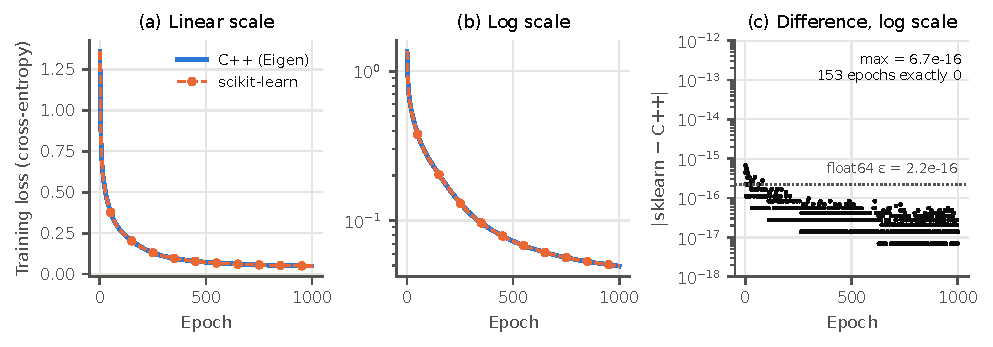
\includegraphics[width=\linewidth]{figures/fig_loss_curves.pdf}
\caption{Curvas de p\'erdida de ambas versiones (a)~en escala lineal y (b)~logar\'itmica, y (c)~su diferencia absoluta. Las curvas son indistinguibles; la diferencia m\'axima es \maxLossDiff{} y en \zeroDiffEpochs{} \'epocas es exactamente nula.}\label{fig:loss}
\end{figure}

Las dos versiones alcanzan la misma calidad (tabla~\ref{tab:resumen}): exactitud de \cppTrainAcc{} en entrenamiento y \cppTestAcc{} en prueba, con p\'erdidas de \cppTrainLoss{} y \cppTestLoss{}, que coinciden con las de \sk (\skTrainLoss{} y \skTestLoss{}). La p\'erdida baja desde \initTrainLoss{} en la primera \'epoca (figura~\ref{fig:loss}). En prueba se clasifican bien \testCorrect{} de \nTest{} muestras; el \'unico tipo de error se ve en la matriz de confusi\'on (figura~\ref{fig:conf}), y las m\'etricas por clase est\'an en la tabla lateral.

\begin{figure}[tbp]\centering
\begin{minipage}[c]{0.46\linewidth}\centering
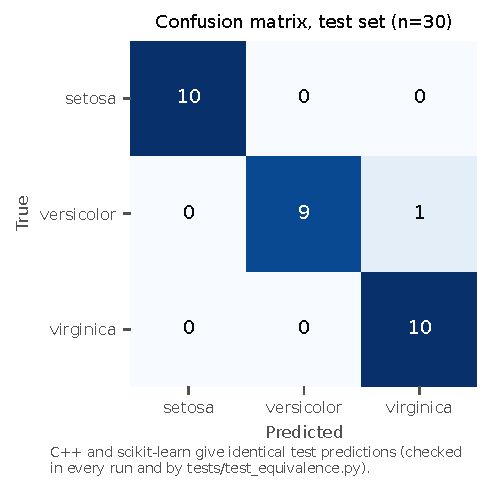
\includegraphics[width=\linewidth]{figures/fig_confusion_matrix.pdf}
\end{minipage}\hfill
\begin{minipage}[c]{0.52\linewidth}\centering\footnotesize
\begin{tabular}{lrrrr}
\toprule
Clase & Precisión & Exhaustividad & F1 & Soporte \\
\midrule
setosa & 1.0000 & 1.0000 & 1.0000 & 10 \\
versicolor & 1.0000 & 0.9000 & 0.9474 & 10 \\
virginica & 0.9091 & 1.0000 & 0.9524 & 10 \\
\bottomrule
\end{tabular}

\end{minipage}
\caption{Matriz de confusi\'on del conjunto de prueba y m\'etricas por clase. Las predicciones de \cpp y \sk son id\'enticas.}\label{fig:conf}
\end{figure}

\begin{table}[tbp]\centering\small
\caption{Resumen de resultados. El \texttt{fit()} de \sk usa \texttt{warm\_start=True} desde los pesos compartidos; el pico de memoria de \sk incluye pandas, que \sk importa por s\'i mismo.}\label{tab:resumen}
\begin{tabular}{lrr}
\toprule
Métrica & C++ (Eigen) & scikit-learn \\
\midrule
\multicolumn{3}{l}{\textit{Calidad}} \\
Exactitud (entrenamiento) & 97.50\% & 97.50\% \\
Exactitud (prueba) & 96.67\% & 96.67\% \\
Pérdida (entrenamiento) & 0.049544 & 0.049544 \\
Pérdida (prueba) & 0.078916 & 0.078916 \\
\midrule
\multicolumn{3}{l}{\textit{Tiempo de entrenamiento (ms, $n=20$ por lado)}} \\
Mediana & 4.35 & 50.75 \\
Media & 4.35 & 50.72 \\
Desv. estándar & 0.09 & 1.11 \\
Mínimo & 4.16 & 48.79 \\
Máximo & 4.49 & 52.39 \\
Aceleración (razón de medianas) & 11.7$\times$ & 1$\times$ \\
Bucle \texttt{partial\_fit}, mediana (mín--máx) & --- & 423.7 (419.2--428.4) \\
\midrule
\multicolumn{3}{l}{\textit{Memoria (mediana y mín--máx, 5 procesos)}} \\
Pico de RSS (MB) & 2.03 (2.02--2.06) & 160 (160--160) \\
Crecimiento del pico en el entrenamiento (KB) & 49.2 (49.2--49.2) & 0 (0--0) \\
\bottomrule
\end{tabular}

\end{table}

\begin{figure}[tbp]\centering
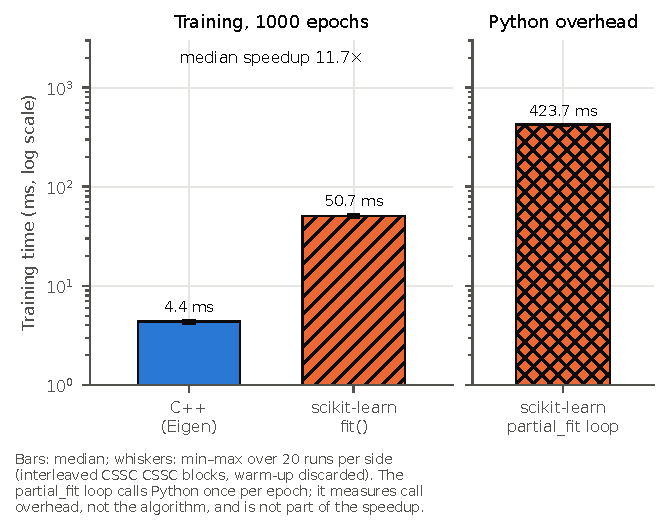
\includegraphics[width=0.62\linewidth]{figures/fig_time.pdf}\\[4pt]
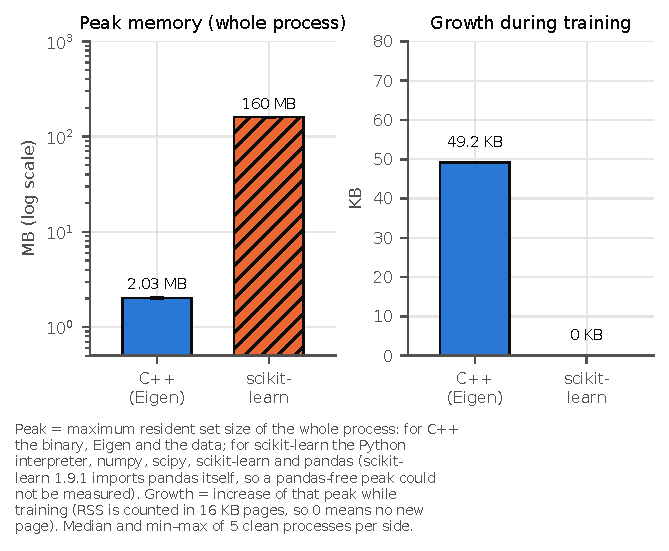
\includegraphics[width=0.62\linewidth]{figures/fig_memory.pdf}
\caption{Tiempo de entrenamiento (mediana y rango m\'in--m\'ax, escala logar\'itmica; el bucle de \texttt{partial\_fit} es sobrecarga de Python) y memoria (pico de todo el proceso y crecimiento durante el entrenamiento).}\label{fig:timemem}
\end{figure}

\section{An\'alisis comparativo}
\paragraph{Rendimiento.} La mediana de entrenamiento es \cppMedianMs{} ms en \cpp y \skMedianMs{} ms en \sk, una aceleraci\'on de \speedupMedian{}$\times$; por \'epoca son \cppPerEpochUs{} y \skPerEpochUs{} $\mu$s. Con \nParams{} par\'ametros y \nTrain{} muestras, cada \'epoca es una cantidad diminuta de c\'alculo, de modo que el tiempo de \sk est\'a dominado por costos fijos por llamada y no por el \'algebra lineal. El bucle de \texttt{partial\_fit} (\partialMedianMs{} ms) es \partialOverFit{}$\times$ m\'as lento que \texttt{fit()} por esa misma raz\'on.

\paragraph{Memoria.} El pico es \cppPeakMB{} MB en \cpp y \skPeakMB{} MB en \sk (\memRatio{} veces). La diferencia es casi enteramente el entorno que \sk necesita (int\'erprete, numpy, scipy, pandas), no la red. En ambos lados el crecimiento durante el entrenamiento es muy peque\~no (\cppGrowthKB{} KB frente a \skGrowthKB{} KB; el RSS se contabiliza en p\'aginas de \pageKB~KB), que son unas pocas p\'aginas. No proviene de reservas durante el entrenamiento: \texttt{noalloc\_check} comprueba que el bucle de \cpp no hace ninguna, y el \texttt{Workspace} y los gradientes ya existen cuando se toma la primera lectura. En mediciones adicionales hechas a mano (no incluidas en la tuber\'ia) el aumento fue el mismo con una, mil y cinco mil \'epocas, apareci\'o por completo en la primera \'epoca y desapareci\'o al ejecutar antes una \'epoca de calentamiento sobre otros buffers; en cambio, tocar de antemano los buffers de la red no lo elimin\'o. Es coherente con p\'aginas de c\'odigo (n\'ucleos de Eigen, funciones matem\'aticas) que el sistema carga la primera vez que se ejecutan, pero no se identific\'o cu\'ales p\'aginas son, as\'i que esa causa es una inferencia y no una medici\'on directa.

\paragraph{Facilidad de implementaci\'on.} La tabla~\ref{tab:loc} cuenta l\'ineas de c\'odigo (sin comentarios ni l\'ineas en blanco, generada por el script que lee el c\'odigo fuente): \locCpp{} en \cpp y \locPython{} en Python, \locRatio{} veces m\'as. Conviene leerla con cuidado: el \'ultimo rengl\'on de Python es c\'odigo \emph{adicional} necesario para la equivalencia, no para usar \sk, y el \cpp incluye la lectura de CSV que Python hace con numpy.

\begin{table}[tbp]\centering\small
\caption{L\'ineas de c\'odigo por componente (no se cuentan la orquestaci\'on, el benchmark ni las pruebas).}\label{tab:loc}
\begin{tabular}{lrr}
\toprule
Componente & C++ (líneas) & Python (líneas) \\
\midrule
Definición del modelo y entrenamiento & 80 & 18 \\
Lectura de datos y pesos desde CSV & 46 & 8 \\
Verificación numérica de gradientes & 46 & --- \\
Equivalencia con C++ (pesos iniciales, warm\_start) & --- & 14 \\
\textbf{Total} & \textbf{172} & \textbf{40} \\
\bottomrule
\end{tabular}

\end{table}

\paragraph{Ventajas y desventajas.}
\begin{itemize}
\item \textbf{\cpp con Eigen.} \emph{Ventajas:} mayor velocidad en este problema, memoria m\'inima, sin dependencia de un int\'erprete, control total del c\'alculo (se puede verificar gradiente y asignaciones) y valor did\'actico. \emph{Desventajas:} m\'as c\'odigo, m\'as superficie de errores (se necesit\'o verificaci\'on num\'erica del gradiente), s\'olo implementa lo que se programa (otra activaci\'on u optimizador implica m\'as c\'odigo) y mayor costo de mantenimiento.
\item \textbf{\sk.} \emph{Ventajas:} el modelo es una llamada de pocas l\'ineas, componentes probados por una gran comunidad, f\'acil de extender (otros solucionadores, validaci\'on cruzada, m\'etricas). \emph{Desventajas:} sobrecarga fija de Python y de validaci\'on, mayor huella de memoria, y menor control: no permite fijar los pesos iniciales sin trucos (secci\'on anterior).
\end{itemize}

\section{Limitaciones}
Las conclusiones deben leerse con estas salvedades:
\begin{itemize}
\item \textbf{Problema diminuto.} Con \nParams{} par\'ametros y \nTrain{} muestras, la aceleraci\'on est\'a dominada por la sobrecarga de Python; no es extrapolable a problemas grandes, donde el costo pasa al \'algebra lineal y la diferencia relativa deber\'ia reducirse (no se midi\'o).
\item \textbf{Conjunto de prueba de \nTest{} muestras.} Cada muestra pesa \testSamplePct{} de exactitud; las diferencias de exactitud con tan pocas muestras no son estad\'isticamente informativas. Adem\'as se usa una sola partici\'on y una sola inicializaci\'on, y no se estudi\'o la variabilidad entre semillas.
\item \textbf{\texttt{warm\_start} en \texttt{fit()}.} El tiempo de \sk parte de pesos ya cargados y excluye la creaci\'on del modelo y la inicializaci\'on aleatoria; el uso t\'ipico (\texttt{fit()} desde cero) no es exactamente lo que se cronometr\'o.
\item \textbf{Pico de memoria de \sk con pandas.} \sk \envSklearn{} importa pandas si est\'a instalado y bloquearlo rompe la biblioteca, por lo que no fue posible medir un pico sin pandas; la cifra incluye pandas, numpy y scipy, y no es el costo de la red.
\item \textbf{Aceleraci\'on variable.} La raz\'on de medianas cambia entre ejecuciones completas: entre \speedupHistMin{}$\times$ y \speedupHistMax{}$\times$ en \nHistoryRuns{} corridas, y entre \speedupBlockMin{}$\times$ y \speedupBlockMax{}$\times$ entre bloques de una misma corrida. Debe citarse como orden de magnitud, no como constante.
\item \textbf{Una sola m\'aquina y compilador.} No se fij\'o el n\'umero de hilos de numpy ni se probaron otros compiladores, sistemas o tama\~nos.
\end{itemize}

\section{Conclusiones y recomendaciones}
Las dos implementaciones son num\'ericamente equivalentes (p\'erdidas, exactitud y predicciones coinciden), por lo que la comparaci\'on de tiempo, memoria y esfuerzo es v\'alida dentro de las limitaciones anteriores. En este problema peque\~no la versi\'on en \cpp es unas \speedupMedian{} veces m\'as r\'apida y usa mucha menos memoria, a costa de \locRatio{} veces m\'as c\'odigo y de la necesidad de verificar el gradiente y las asignaciones.

\textbf{Recomendaciones.} (i) Para prototipado, investigaci\'on y la mayor\'ia de problemas tabulares peque\~nos o medianos, usar \sk: el costo de desarrollo domina al costo de ejecuci\'on. (ii) Elegir una implementaci\'on propia en \cpp cuando importen la latencia, la ausencia de un int\'erprete, la huella de memoria o el control del c\'alculo, y mantener como pruebas la verificaci\'on del gradiente y la comparaci\'on con una referencia. (iii) Al comparar tiempos, igualar primero el c\'alculo (datos, pesos, hiperpar\'ametros, punto de medida) y medir con repeticiones, calentamiento y orden intercalado. \emph{Trabajo futuro:} conjuntos m\'as grandes, varias semillas, mini-lotes, control de hilos y otros compiladores.

\bibliographystyle{unsrt}
\bibliography{references}
\end{document}
